\documentclass[course=eragp]{aspdoc}

\usepackage{xstring}
\usepackage{catchfile}
\usepackage{amsmath}
\usepackage{amsfonts}
\usepackage{amssymb}
\usepackage{graphicx}
\usepackage{booktabs}
\usepackage{icomma}
\usepackage{siunitx}
\usepackage{multicol}
\usepackage{verbatim}
\usepackage{url}
\usepackage{caption}
\usepackage{subcaption}
\usepackage[german]{varioref}
\usepackage[toc]{appendix}
\usepackage{tikz}
\usepackage{pgfplots}

\author{Noah Dormann \and Simon Kammermeier \and Johannes Pfannschmidt \and Florian Schmidt}
\date{Summer term 2020}
\title{Dynamic Binary Translation for RISC--V code on x86--64}

% ======= NOTE =======
% Checkout todos (--> remove before flight).
% Many unresolved issues/missing details/pending layout
% are marked by todos. Be sure to resolve all prior to
% submission.
% Hint fixes for the layout when the text is finalised.
% Until then, the floats may float.
% ====================

% typeset current git commit id for drafts
% todo remove commit id before submission
\CatchFileDef{\headfull}{../../.git/HEAD}{}
\StrGobbleRight{\headfull}{1}[\head]
\StrBehind[2]{\head}{/}[\branch]
\CatchFileDef{\commit}{../../.git/refs/heads/\branch}{}
\cfoot{Draft after commit \commit on branch \branch.}

% define utilities and symbols
\newcommand*\diff{\mathop{}\!\mathrm{d}}
\newcommand*\Diff[1]{\mathop{}\!\mathrm{d^#1}}
\newcommand{\define}[2]{\item \textbf{#1}\\#2}
\newcommand{\conclude}[0]{\ensuremath{\Longrightarrow} }
\newcommand{\refer}[0]{\ensuremath{\rightarrow} }
\sisetup{range-phrase=--,range-units=single}
\MakeOuterQuote{"}

% list sections and subsections in toc, ignore smaller
\setcounter{tocdepth}{2}

% itemize without parskip and itemsep for compact listings
\newenvironment{itemize*}%
  {\begin{itemize}%
    \setlength{\itemsep}{0ex}%
    \setlength{\parskip}{0ex}}%
  {\end{itemize}}

% environment setup for pgfplots and tikz
\pgfplotsset{compat=newest}
\definecolor{era-qemu}{HTML}{FFB74D}
\definecolor{era-dbt-1}{HTML}{f44336}
\definecolor{era-dbt-2}{HTML}{64B5F6}
\definecolor{era-native}{HTML}{AED581}

\begin{document}
\maketitle
\tableofcontents
\pagebreak

% \input separate files for every section! --> avoids merge conflicts

\section{Introduction}
RISC-V is an open ISA first conceptualised in 2010 with the initial goals of research and education in mind.
In contrast to Intel's x86~\cite{intel2017man} it employs the RISC (Reduced Instruction Set Computer) scheme by providing fewer and less powerful instructions, addressing modes and cycle-heavy features in favour of a simplified microarchitecture.
Its development takes the lessons learned in terms of backwards compatibility and future-proofing from other widespread ISAs like x86 into account, and aims to provide an open interface for the architecture, rather than strict implementation details.
This grants a large freedom to the implementors and greatly increases the flexibility and ease of working with the architecture~\cite[S. 1f]{riscvspec}.
As such, it looks to be open to future extensions by already defining a basis for future 128-bit integer instructions and instruction length encodings of up to 176 bits (22 bytes).
The possibility to expand further when widespread technology developments would require such an expansion is also remained open.


\subsection{Problem description}
There is already some hardware available for RISC-V\footnote{The biggest name here is probably SIFive~\cite{sifive}, which already produce multi-core CPUs with super scalar out-of-order pipelines reaching multi-GHz clock speeds.}, but it is not yet widespread.
Developers usually don't have access to real hardware, so they must instead rely on emulation to test their code written for the RISC-V platform.

\paragraph{Modes of binary translation}
When attempting to execute guest programs compiled for a foreign architecture on a different native one, there are essentially three distinct approaches at one's disposal.

The main principles to achieve this are:
\begin{itemize}
    \item \textbf{Interpretation}, where, much alike interpreted programming languages (e.g.\ JavaScript, Python, or Ruby), the assembly instructions located in the binary are examined while emulating the execution of the program, and equivalent actions are taken on the host system in order to simulate the guest ISA\@.
        \subitem While likely being the easiest to actually be implemented, this comes with a significant performance penalty mainly because every single assembly instruction will have to be interpreted for every execution of that program part, potentially causing a lot of redundant work.
    \item \textbf{Static Binary Translation}, where the guest executable is statically reverse-engineered and translated to the host architecture as a whole.
    After this translation step, it can be executed as if it were a native binary, without the need for any further special treatment.
    In theory you could reach near native speeds for the generated binary using this technique.
    There some hurdles with this though, one example is register indirect branches, which require some way to convert the guest addresses to native at runtime.
    Any program that produces or edits assembly at runtime would also generally prove difficult to translate statically.
    \item \textbf{Dynamic Binary Translation} (DBT), which serves as a middle ground between interpreting and statically translating the executable.
    It aims to translate the program on the fly, while only focussing on the parts that are actually needed for execution.
    Therefore, it can save some of the overhead of a static translator by not spending execution time on unused code paths.
    The other aforementioned issues are also fairly easily resolved.
    Unlike an interpreter, every instruction only has to be translated once and can then be run without any unnecessary overhead.
    Of course, this assumes that the translation routines are relatively swift in performing their functions, so as not to introduce any more overhead than necessary~\cite[S. 1f.]{bintrans}.
\end{itemize}

\subsection{Motivation}
% todo ISA == guest and host architectures? why twice?
One of the most popular software emulators in general is QEMU~\cite{bellard2005qemu}\@.
While QEMU is a portable DBT that supports a wide variety of guest and host architectures and ISAs, this also makes it hard to optimise it for a specific guest/host combination and therefore the program execution will be slower than necessary.

Our aim is to provide a faster emulator, allowing the execution of RISC-V code on an x86-64 machine by means of dynamic binary translation.

















\section{Approach}
In the following, the term \textit{host} will refer to the system of the native architecture the binary translator is built for (in our case, x86-64), and the term \textit{guest} will designate the foreign system we are attempting to emulate (RISC--V).


\subsection{Modes of binary translation}

When attempting to execute guest programs compiled for a foreign architecture on a different native one, there are essentially three distinct approaches at one's disposal.

The two extremes of this spectrum are:
\begin{itemize}
	\item \textbf{Interpretation}, where, much alike interpreted programming languages (e. g. JavaScript, Python, or Ruby), the assembly instructions located in the binary are examined while emulating the execution of the program, and equivalent actions are taken on the host system in order to simulate the guest ISA.
	\item \textbf{Static Binary Translation}, where the guest executable is statically reverse-engineered and translated to the guest architecture as a whole.
	After this translation step, it can be executed as if it were a native binary, without the need for any further special treatment.
\end{itemize}

However, it turns out both of these approaches have their downsides.
Interpretation, on the one hand, comes with a significant performance penalty.
Just as programs written for interpreted languages like Python will always execute more slowly than equivalent programs created with a compiled language like C++, there is a large overhead to having to interpret every single instruction in an executable binary.
Especially if the program contains certain parts of the code that are executed many times -- bodies of large loop statements, for example -- the interpreter has to do a lot of redundant work in simulating the same instruction operations for as many times as that section is called.

Static binary translation, on the other hand, is very difficult to achieve correctly.
If done well, it would produce a binary native to the host's environment, and could thus run without any wrapper programs or other utilities, enjoying the same performance benefits as other native executables do.

However, there are certain programming concepts that have proven difficult for a static binary translator to deal with.
Register indirect branching, for example, is one of them, where the jump address is not selected statically, but rather computed at runtime.
Deducing the jump target would thus again require (in some ways) emulating the program execution in order to know the values needed for the computation.
In light of the project at hand, a dynamic binary translator would also be a very difficult program to translate statically, due to the fact that it generates some the code it executes at runtime.

The solution to these issues, and our chosen approach for this project, is
\begin{itemize}
	\item \textbf{Dynamic Binary Translation}, which serves as a middleground between interpreting and statically translating the executable.
	It aims to translate the program on the fly, while only focussing on the parts that are actually needed for execution.
\end{itemize}

By only translating the parts of the binary that are actually executed, the dynamic binary translator (DBT) can save the overhead a static translator would have spent on translating unused code paths.
Also, as the DBT is actually stepping through and executing the program, the other limitations of static binary translators essentially do not apply.

It can also perform significantly better than an interpreter might, as it has to translate a single piece of code only once, which can then be called many times; unlike the above-mentioned behaviour of an interpreter.
Furthermore, as it produces blocks of code that are native to the host platform, it can be reasonably expected that a single block's execution will be faster than the respective emulation.

Of course, this assumes that the translation routines of the DBT are relatively swift in performing their functions, so as not to introduce any more overhead than absolutely necessary.


\subsection{Partitioning the input code}
Logically, the DBT must somehow divide the code into chunks it can then process for translation and execution.

%todo continued about basic blocks, jump/call instructions, etc.















\section{Implementation Details}
The following section aims to provide an in-depth overview of the system's architecture as well as the rationale for major design decisions taken during the implementation.

\subsection{System architecture and execution control flow}
% todo overview, add class diagrams and flow charts

\subsection{Instruction translation process}
% todo

\subsection{Code cache and TLB for block lookup}
% todo

\subsection{Static hybrid register mapping}
% todo register mapping details

\subsection{Optimisation of the generated code}
\subsubsection{Block chaining}
\subsubsection{Recursive jump translation}
\subsubsection{Macro operation fusion}
% todo optimisation details, maybe split up? more sections?

\subsection{Detailed system call overview}
% todo special description for emulated calls

As described in section \vref{sec:syscall-handling}, we must assume the role of the kernel by handling system calls during the execution of the guest program.
We achieve this by translating the \texttt{ECALL} instruction as a context switch and jump to the \texttt{emulate\_ecall} routine in the DBT, which can then take the appropriate action.

As we stored the guest's registers before jumping to the handler, the requested system call index is now available to the DBT in the register file as entry \texttt{a7}, as per the RISC-V standard calling convention.
We may now handle the system calls based on that index and the arguments passed in the registers \texttt{a0} through \texttt{a6}, and write the return value to entry \texttt{a0} of the register file prior to switching the context back to the guest.

As previously mentioned, some system calls require special handling when encountered by the DBT (see table \vref{tab:syscall-special} for details).
The following will describe the specifics of these issues with system calls that are either not present on the x86-64 host architecture, or may influence or break the state of the DBT.
\begin{description}
	\item[Adapting structure data format.]
	There are system calls like \texttt{fstat} and \texttt{fstatat} that exist both on RISC-V as well as x86-64, but use different data structure layouts in their return values.
	Thus, the DBT must adapt the host's returned data to the required format prior to passing it back to the guest.
	
	
	\item[Emulation required.]
	The DBT captures the \texttt{exit} and \texttt{exit\_group} calls.
	Passing them through would immediately terminate the DBT -- an action that is undesirable as it prevents any form of clean-up or post-execution profiling and analysis to take place.
	Thus, the DBT uses these system calls to set a flag which stops the translator's main loop from executing the next iteration.
	
	The \texttt{brk} system call must also be entirely emulated, as it would otherwise allow the guest program to modify the endpoint of the DBT's data segment (\textit{program break}), thus potentially deallocating some of the translator's memory.
	
	
	\item[Ignoring system calls.]
	% todo expand the rationale here. is this correct?
	The \texttt{rt\_sigaction} system call is ignored by the DBT, as any signals received by the process will be handled by the translator due to the fact that the guest program's execution is emulated in the DBT's process.
	
	
	\item[Guarded pass-through to host.]
	Essentially, any system call that has the possibility to influence the state or memory of the translator needs to have respective safe-guards in place.
	A good example of this behaviour is the \texttt{mmap} system call, the handling of which also reflects the memory layout scheme discussed in section \vref{sec:memory-layout}.
	
	In any case, we must prevent a memory mapping into the translator's memory region.
	Mappings that do not interfere with the DBT's memory can be passed along to the host directly.
	In case a hinted mapping would conflict with the translator's memory, we may just re-hint the mapping to the top of the guest's address space.
	When the call is not hinted (the \texttt{MAP\_FIXED} or \texttt{MAP\_FIXED\_NOREPLACE} flag commands the mapping at exactly the specified address), we are unable to provide the guest with the requested mapping; thus we simulate an existing mapping in the location in question by returning \texttt{EEXIST} for \texttt{MAP\_FIXED\_NOREPLACE} and failing the call with \texttt{EINVAL} for \texttt{MAP\_FIXED}.
	
	Similarly, we fail the guest's \texttt{munmap} with \texttt{EINVAL} in cases where the translator's memory would be compromised by the deallocation.
\end{description}

The other supported system calls may be directly passed through to the host after performing the necessary index mapping (see table \vref{tab:syscall-pass-through}).

\begin{table}
	\centering
	\begin{tabular}{ccc}
		\toprule
		\textbf{System Call (index)} & \textbf{Handling} & \textbf{x86-64 base (index)}\\ 
		\midrule
		\texttt{fstatat} (79) & data reformat & \texttt{newfstatat} (262)\\
		\texttt{fstat} (80) & data reformat & \texttt{fstat} (5)\\
		\texttt{exit} (93) & emulate & n/a\\
		\texttt{exit\_group} (94) & emulate & n/a\\
		\texttt{rt\_sigaction} (134) & ignore & n/a\\
		\texttt{brk} (214) & emulate & n/a\\
		\texttt{munmap} (215) & guarded pass-through & \texttt{munmap} (11)\\
		\texttt{mmap} (222) & guarded pass-through & \texttt{mmap} (9)\\
		\bottomrule
	\end{tabular}
	% todo keep up-to-date
	% state: aa55cef4816eb790df21f4742b7cf1f29685da49
	\caption{An overview of the system calls we support that require special handling by the binary translator.}
	\label{tab:syscall-special}
\end{table}

\begin{table}
	\centering
	\begin{tabular}{rlc}
		\toprule
		\textbf{RISC-V system call} & \textbf{\ldots index} & \textbf{x86-64 index}\\
		\midrule
		\texttt{getcwd} & 17 & \refer 79\\
		\texttt{fcntl} & 25 & \refer 72\\
		\texttt{ioctl} & 29 & \refer 16\\
		\texttt{unlinkat} & 35 & \refer 263\\
		\texttt{faccessat} & 48 & \refer 269\\
		\texttt{chdir} & 49 & \refer 80\\
		\texttt{fchmod} & 52 & \refer 91\\
		\texttt{fchown} & 55 & \refer 93\\
		\texttt{pipe2} & 59 & \refer 293\\
		\texttt{openat} & 56 & \refer 257\\
		\texttt{close} & 57 & \refer 3\\
		\texttt{getdents64} & 61 & \refer 217\\
		\texttt{lseek} & 62 & \refer 8\\
		\texttt{read} & 63 & \refer 0\\
		\texttt{write} & 64 & \refer 1\\
		\texttt{writev} & 66 & \refer 20\\
		\texttt{readlinkat} & 78 & \refer 267\\
		\texttt{utimensat} & 88 & \refer 280\\
		\texttt{set\_tid\_address} & 96 & \refer 218\\
		\texttt{futex} & 98 & \refer 202\\
		\texttt{set\_robust\_list} & 99 & \refer 273\\
		\texttt{clock\_gettime} & 113 & \refer 228\\
		\texttt{tgkill} & 131 & \refer 234\\
		\texttt{rt\_sigprocmask} & 135 & \refer 14\\
		\texttt{uname} & 160 & \refer 63\\
		\texttt{gettimeofday} & 169 & \refer 96\\
		\texttt{getpid} & 172 & \refer 39\\
		\texttt{getuid} & 174 & \refer 102\\
		\texttt{geteuid} & 175 & \refer 107\\
		\texttt{getgid} & 176 & \refer 104\\
		\texttt{getegid} & 177 & \refer 108\\
		\texttt{gettid} & 178 & \refer 186\\
		\texttt{sysinfo} & 179 & \refer 99\\
		\texttt{execve} & 221 & \refer 59\\
		\texttt{wait4} & 260 & \refer 61\\
		\texttt{prlimit64} & 261 & \refer 302\\
		\texttt{renameat2} & 276 & \refer 316\\
		\texttt{getrandom} & 278 & \refer 318\\
		\bottomrule
	\end{tabular}
	% todo keep up-to-date
	% state: aa55cef4816eb790df21f4742b7cf1f29685da49
	\caption{An overview of the system calls handled via pass-through to the host.}
	\label{tab:syscall-pass-through}
\end{table}










\section{Results and Performance}
% todo expand this section with further details

\begin{comment}
% ======= EXAMPLE PLOT =======
% Update, copy and modify as needed. Shows tikz usage.
% todo remove before submission (obviously).
% ============================
% The [h] requests TeX put the float <h>ere.
% There are other options for <p>age, <t>op, <b>ottom;
% If it shouldn't float, \usepackage{float} and use [H]
% or a minipage with associated caption.
\begin{figure}[h]
	\centering
	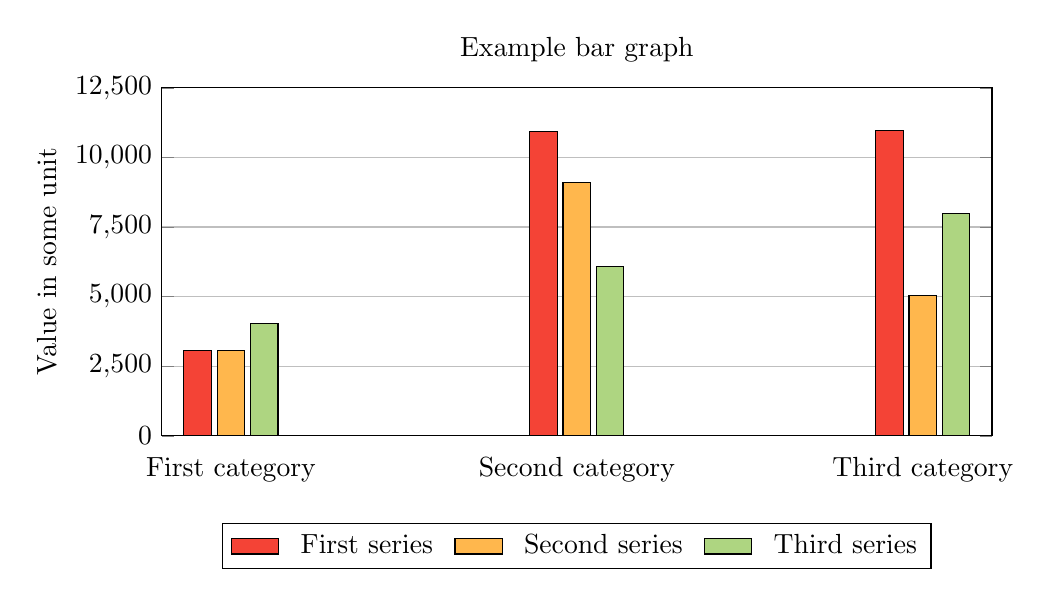
\begin{tikzpicture}
		\begin{axis}[%
			title = {Example bar graph},
			ybar,
			area legend,
			ylabel = {Value in some unit},
			xtick = data,
			xtick style = {draw = none},
			ytick = {0, 2500, 5000, 7500, 10000, 12500},
			scaled y ticks = false,
			symbolic x coords={First category, Second category, Third category},
			ymin = 0, ymax = 12500,
			ymajorgrids = true,
			height = 6.0cm,
			width = \linewidth,
			legend style = {
				at = {(0.5, -0.25)},
				anchor = north,
				legend columns = 3,
				column sep = 0.2cm
			}
		]	
			\addplot+ [
				fill=era-dbt-1,
				draw=black
			] coordinates {
				(First category, 3061)
				(Second category, 10930)
				(Third category, 10971)
			};
			
			\addplot+ [
				fill=era-qemu,
				draw=black
			] coordinates {
				(First category, 3061)
				(Second category, 9092)
				(Third category, 5042)
			};
			
			\addplot+ [
				fill=era-native,
				draw=black
			] coordinates {
				(First category, 4043)
				(Second category, 6092)
				(Third category, 7971)
			};

			
			\legend{First series, Second series, Third series}
		\end{axis}
	\end{tikzpicture}
	\caption{I am an example figure. If you're reading the submitted document, someone forgot to remove me.}
\end{figure}
\end{comment}


Measuring the performance of the DBT was accomplished by using the tools in \textit{SPEC CPU 2017}'s \texttt{intspeed} suite of benchmarks.
This not only generates reproducible and widely accepted results in the industry, it also validates the results produced during the run, thus ruling out any errors in the benchmark's translation.

% todo include benchmark description table (and list of tables) for the spec programs with the benchmark workload description
The \texttt{intspeed} suite also presents a variety of different workloads to the translator that are based on real-life scenarios, thus producing an accurate and understandable overview of the DBT's performance in a non-controlled environment.
Further context is provided by performance testing using the data compression utility \textit{gzip}~\cite{gzip}, where compression time is compared between runs on a native machine, in QEMU and in the DBT.

All testing was performed on an x86--64 8-core \textit{Intel Xeon Bronze 3106} system clocked at $1,70$ GHz base with $78$ GiB of physical memory, running \textit{Ubuntu 18.04.3 LTS}, kernel version \textit{4.15.0-70-generic}.
The DBT was compiled via \texttt{CMAKE\_BUILD\_TYPE} set to \texttt{Release}, which implies \texttt{-O3}.

\subsection{SPEC CPU 2017 Results}
% todo benchmark results


% ======= SPEC CPU Results =======
% Results of the intspeed SPEC CPU 2017 runs.
% todo Keep up to date with performance-improving changes.
% todo normalise the results
% ================================
\begin{figure}[h]
	\centering
	% 1/2
	\begin{subfigure}[b]{\textwidth}
		\centering
		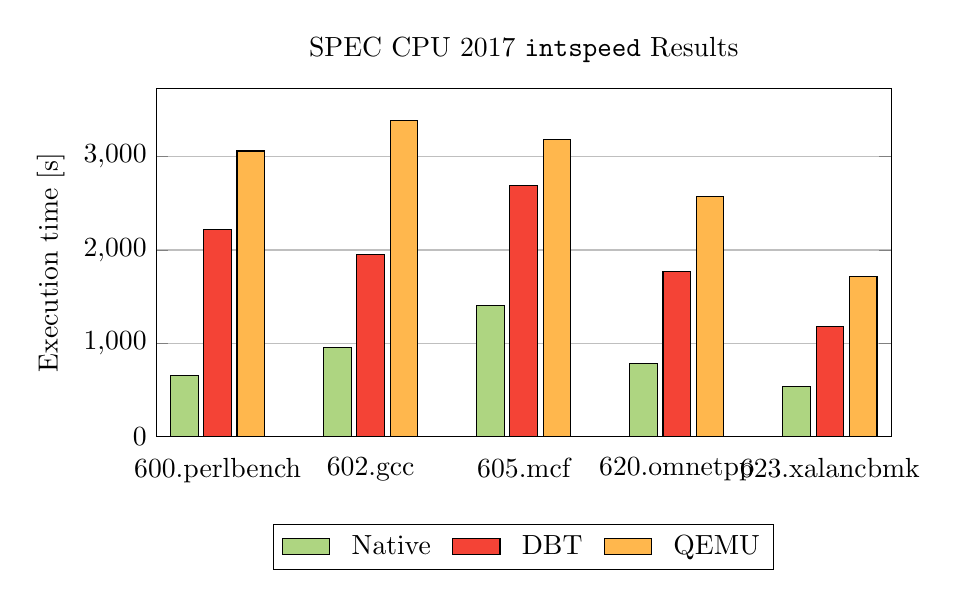
\begin{tikzpicture}
			\begin{axis}[%
				title = {SPEC CPU 2017 \texttt{intspeed} Results},
				ybar,
				area legend,
				ylabel = {Execution time [s]},
				xtick = data,
				xtick style = {draw = none},
				scaled y ticks = false,
				symbolic x coords={600.perlbench, 602.gcc, 605.mcf, 620.omnetpp, 623.xalancbmk},
				ymin = 0,
				ymajorgrids = true,
				height = 6.0cm,
				width = 0.9\linewidth,
				legend style = {
					at = {(0.5, -0.25)},
					anchor = north,
					legend columns = 3,
					column sep = 0.2cm
				}
			]	
				% Native results
				\addplot+ [
					fill=era-native,
					draw=black
				] coordinates {
					(600.perlbench, 654)
					(602.gcc, 953)
					(605.mcf, 1409)
					(620.omnetpp, 779)
					(623.xalancbmk, 533)
				};
				
				% DBT results
				\addplot+ [
					fill=era-dbt-1,
					draw=black
				] coordinates {
					(600.perlbench, 2222)
					(602.gcc, 1956)
					(605.mcf, 2695)
					(620.omnetpp, 1768)
					(623.xalancbmk, 1178)
				};
				
				% QEMU results
				\addplot+ [
					fill=era-qemu,
					draw=black
				] coordinates {
					(600.perlbench, 3061)
					(602.gcc, 3390)
					(605.mcf, 3182)
					(620.omnetpp, 2576)
					(623.xalancbmk, 1711)
				};
	
				\legend{Native, DBT, QEMU}
			\end{axis}
		\end{tikzpicture}
		\caption	{Partial benchmark results.}
	\end{subfigure}
	
	% 2/2
	\begin{subfigure}[b]{\textwidth}
		\centering
		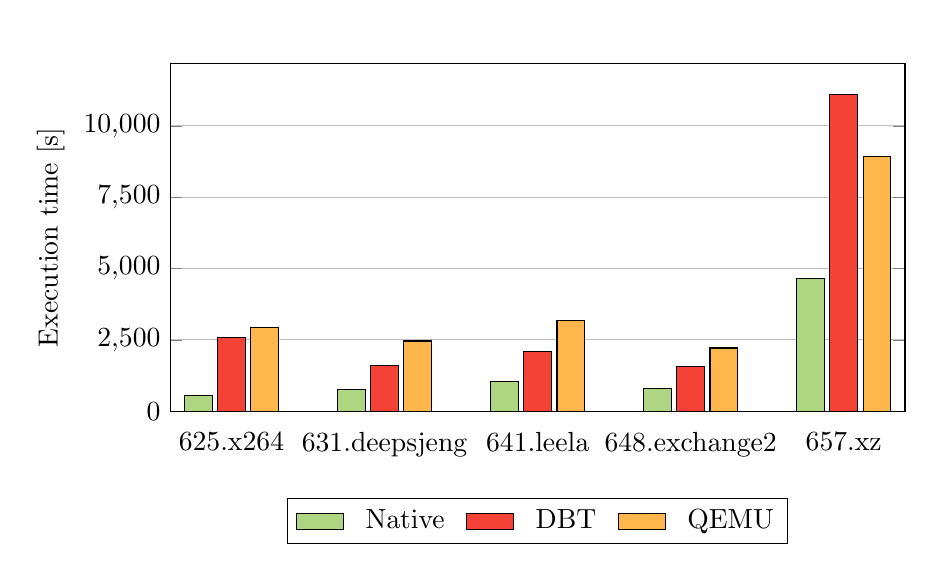
\begin{tikzpicture}
			\begin{axis}[%
				title = {~},
				ybar,
				area legend,
				ylabel = {Execution time [s]},
				xtick = data,
				xtick style = {draw = none},
				ytick = {0, 2500, 5000, 7500, 10000, 12500, 15000},
				scaled y ticks = false,
				symbolic x coords={625.x264, 631.deepsjeng, 641.leela, 648.exchange2, 657.xz},
				ymin = 0,
				ymajorgrids = true,
				height = 6.0cm,
				width = 0.9\linewidth,
				legend style = {
					at = {(0.5, -0.25)},
					anchor = north,
					legend columns = 3,
					column sep = 0.2cm
				}
			]	
				% Native results
				\addplot+ [
					fill=era-native,
					draw=black
				] coordinates {
					(625.x264, 554)
					(631.deepsjeng, 773)
					(641.leela, 1045)
					(648.exchange2, 780)
					(657.xz, 4665)
				};
				
				% DBT results
				\addplot+ [
					fill=era-dbt-1,
					draw=black
				] coordinates {
					(625.x264, 2590)
					(631.deepsjeng, 1603)
					(641.leela, 2080)
					(648.exchange2, 1575)
					(657.xz, 11083)
				};
				
				% QEMU results
				\addplot+ [
					fill=era-qemu,
					draw=black
				] coordinates {
					(625.x264, 2921)
					(631.deepsjeng, 2459)
					(641.leela, 3171)
					(648.exchange2, 2213)
					(657.xz, 8915)
				};

				\legend{Native, DBT, QEMU}
			\end{axis}
		\end{tikzpicture}
		\caption	{Partial benchmark results.}
	\end{subfigure}
	\caption[SPEC CPU 2017 Results]%
	{Results of \texttt{ref}-workload runs of \textit{SPEC CPU 2017}'s \texttt{intspeed}.}
\end{figure}
% ================================

\subsection{Data compression via gzip}
% gzip results
Next to the results of the \textit{SPEC CPU 2017} suite, it is also valuable to measure the performance of the translator in real-world workloads by running data compression via \textit{gzip}.

The native \textit{gzip} binary for the reference runs was obtained from the default package repositories.
As there is no such executable available for the RISC-V architecture, the sources had to be manually compiled.
% todo Simon? insert info here about compile settings for risc_gzip

% ======= gzip execution time =======
% Execution time of compression (500 MB, 10 runs).
% todo keep up-to-date with performance improvements
% ===================================
\begin{figure}[h]
	\centering
	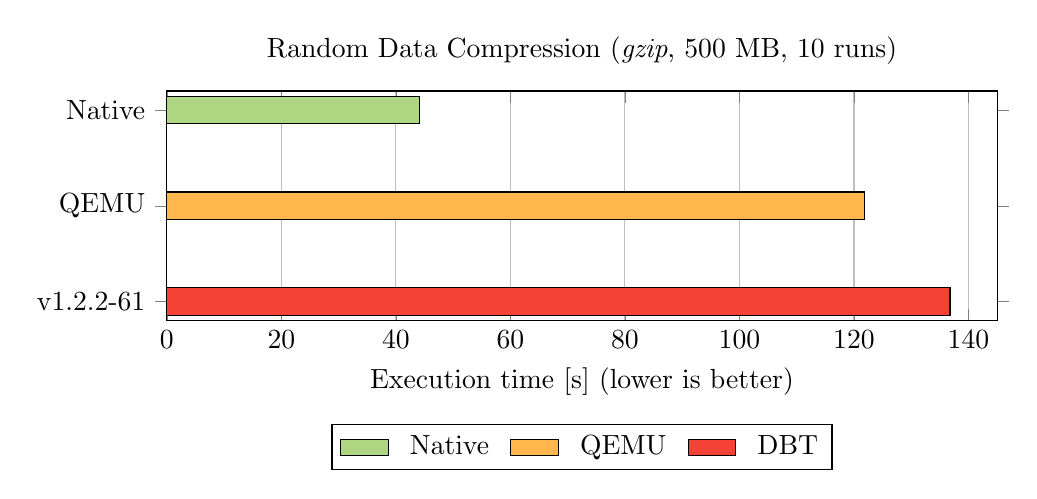
\begin{tikzpicture}
		\begin{axis}[%
			title = {Random Data Compression (\textit{gzip}, 500 MB, 10 runs)},
			xbar,
			area legend,
			xlabel = {Execution time [s] (lower is better)},
			symbolic y coords = {Native,QEMU,v1.2.2-61},
			xmin = 0, xmax = 145,
			bar shift = 0.0cm,
			y dir = reverse,
			xmajorgrids = true,
			height = 4.5cm,
			width = \linewidth,
			legend style = {
				at = {(0.5, -0.45)},
				anchor = north,
				legend columns = 3,
				column sep = 0.2cm
			}
		]	
			\addplot+ [
				fill=era-native,
				draw=black
			] coordinates {
				(44.14,Native)
			};

			\addplot+ [
				fill=era-qemu,
				draw=black
			] coordinates {
				(121.83,QEMU)
			};
			
			\addplot+ [
				fill=era-dbt-1,
				draw=black
			] coordinates {
				(136.77,v1.2.2-61)
			};
			
			\legend{Native, QEMU, DBT}
		\end{axis}
	\end{tikzpicture}
	\caption[Execution time of gzip compression (500 MB, 10 runs)]%
	{Execution time of gzip file compression (500 MB of random data, 10 runs) in seconds (lower is better).}
	\label{fig:gzip-execution-time}
\end{figure}
% ===================================

Figure \vref{fig:gzip-execution-time} lists the execution times of \textit{gzip} compressing a pseudo-random $500$ MB file sourced from \texttt{/dev/urandom}\footnote{Reproducible via \texttt{base64 /dev/urandom | head -c 524288000 > random.txt;}}.
% todo add analysis as soon as results are finalized

\subsection{Other performance metrics}
By implementing optimisations to the DBT like a return address stack, recursive jump target translation and block chaining as discussed in section \vref{sec:optimise}, we are able to meaningfully increase the performance of the translator in certain workloads, to the point where we outperform \textit{QEMU} significantly.

% ======= merge_sort execution time =======
% Execution time of the merge_sort test.
% todo keep up-to-date with performance improvements
% =========================================
\begin{figure}[h]
	\centering
	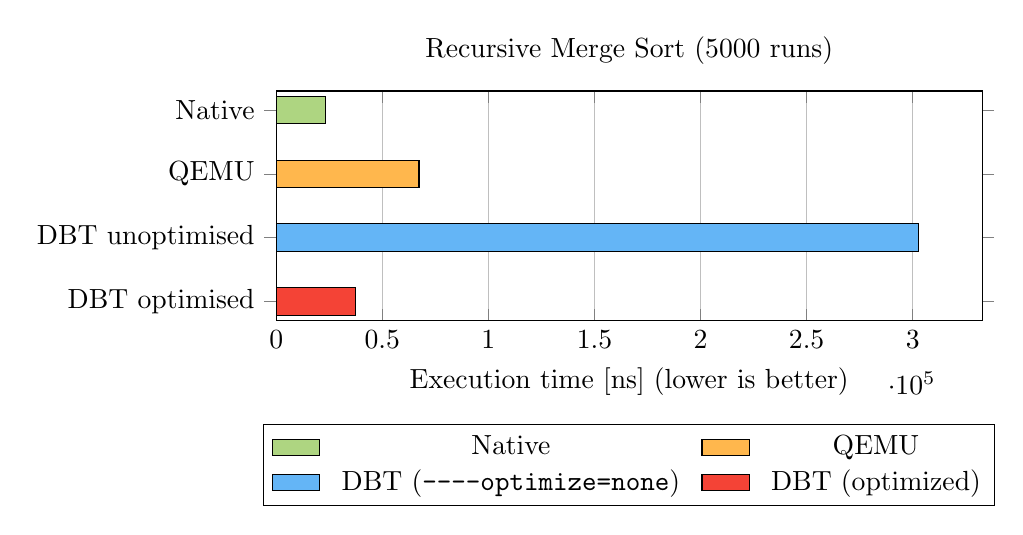
\begin{tikzpicture}
		\begin{axis}[%
			title = {Recursive Merge Sort (5000 runs)},
			xbar,
			area legend,
			xlabel = {Execution time [ns] (lower is better)},
			symbolic y coords = {Native,QEMU,DBT unoptimised,DBT optimised},
			xmin = 0,
			bar shift = 0.0cm,
			y dir = reverse,
			xmajorgrids = true,
			height = 4.5cm,
			width = 0.87\linewidth,
			legend style = {
				at = {(0.5, -0.45)},
				anchor = north,
				legend columns = 2,
				column sep = 0.2cm
			}
		]	
			\addplot+ [
				fill=era-native,
				draw=black
			] coordinates {
				(23385.65,Native)
			};

			\addplot+ [
				fill=era-qemu,
				draw=black
			] coordinates {
				(67312.47,QEMU)
			};
			
			\addplot+ [
				fill=era-dbt-2,
				draw=black
			] coordinates {
				(302521.38,DBT unoptimised)
			};
			
			\addplot+ [
				fill=era-dbt-1,
				draw=black
			] coordinates {
				(37565.99,DBT optimised)
			};
			
			\legend{Native, QEMU, DBT (\texttt{----optimize=none}), DBT (optimized)}
		\end{axis}
	\end{tikzpicture}
	\caption[Execution time of merge sort (5000 runs)]%
	{Execution time of merge sort (5000 runs) in nanoseconds (lower is better). Testing performed with v1.2.2-61.}
	\label{fig:dbt-optimisations}
\end{figure}
% =========================================

Figure \vref{fig:dbt-optimisations} shows a manifestation of these performance gains, as seen by executing a benchmark based on a recursive implementation of the merge sort algorithm.
























\section{Summary}
% todo
Summary here\ldots

\newpage
\section*{Appendices}
\begin{appendices}	
	\renewcommand\thesubsection{\Alph{subsection}}
	\section{Download and installation instructions}
The source code for the translator can be downloaded by checking out the project's git repository.
Take care to either \texttt{git clone} the repository with the option flag \texttt{--recursive}, or to run the command
\begin{lstlisting}
	git submodule update --init
\end{lstlisting}
as the repository contains submodules that are required for compilation.

Then, the translator can be built by exeucting
\begin{lstlisting}
	sudo apt-get -y install gcc g++ cmake make autoconf meson
	mkdir build && cd build && cmake .. && make
\end{lstlisting}
in the root directory of the repository.
Note that the build requires CMake version 3.16 or above.
This will build two artifacts:
\begin{description}
	\item[translator] The actual dynamic binary translator.
	For details on the usage, see section \vref{sec:translator-usage}, or execute \texttt{./translator -h}.
	
	\item[test] The unit test binary.
	It can be executed via \texttt{./test} and performs extensive unit testing of the RISC-V instruction implementations, the cache, register file, as well as the parser.
\end{description}

\section{Executable program requirements}
We can execute binaries compiled via the tools provided in the RISC-V GNU toolchain\footnote{For further information as well as download and usage instructions, see \url{https://github.com/riscv/riscv-gnu-toolchain} (last accessed on 25.09.2020).}.
The executables need to be linked statically (pass the flag \texttt{-static} to gcc when compiling), as the translator does not support dynamically linked files.

% todo update if floating point comes into play
We currently support binaries compiled for the architecture specifier \texttt{rv64ima}, meaning the compiler is free to utilise the base integer instruction set (\texttt{i}), as well as the instructions provided by the multiplication (\texttt{m}) and atomic standard extensions (\texttt{a}).
This can be achieved by passing \texttt{-march=rv64ima} to gcc\footnote{Note that some architecture strings require recompilation of the toolchain. Also, the aforementioned option implies \texttt{-mabi=lp64}.}.


\section{Using the translator}
\label{sec:translator-usage}
% this assumes the state of opt_rewrite, todo update as necessary
\begin{lstlisting}
	./translator [translator option(s)] -f <filename> [guest options]
\end{lstlisting}

Seen above is the syntax for executing the translator with a guest program.
All possible translator options are described in the help text, as seen by executing \texttt{./translator -h}.
Every option after the filename specified via the \texttt{-f} flag is passed along to the guest in its \texttt{argv}, so all options intended for the translator must be passed before \texttt{-f}.

The command line options also include the ability to analyse (\texttt{-a}) the binary to produce a detailed breakdown of which instruction mnemonics and registers the guest will use when executed.
Furthermore, it includes the ability to time the execution of only the guest program by passing the flag \texttt{-b}.

Logging can be controlled by passing the requested category to the \texttt{----log} flag as detailed in the help, and can provide insights into the state of the translator during execution or debugging.
Lastly, it is also possible to selectively disarm optimisation features like the return address stack, block chaining or recursive jump target translation via \texttt{----optimize}.


\section{Using the bundled tools}
% todo section about usage of -a, -p, -b and --perf
There seems to be nothing here yet\ldots










\end{appendices}

\newpage
\listoftables
\listoffigures

\newpage
\bibliographystyle{ieeetr}
\addcontentsline{toc}{section}{References}
\bibliography{paper}{}
\end{document}
